\documentclass[a4paper,oneside]{book}   % list options between brackets
\usepackage{graphicx}              % list packages between braces
\graphicspath{{graphics/}}
\usepackage{url}

% type user-defined commands here

\begin{document}

\title{A Proposal for an  Open Wireless Sensor Network On-Line Course} % Title of the book
\author{Jaume Barcelo et al.} % Author
\date{\today}    % type date between braces

\maketitle % Print the title page
\tableofcontents

\chapter{Project Report}
\section{Introduction and goals} % The asterisk leaves out this chapter from the table of contents

It is a commonplace that the Internet is changing our lives.
It is changing the way we learn and also the way we contribute to our communities and organize ourselves.
It is our goal to use the network to teach about the construction of new networks.
In this course we will explore the bottom-up creation of a wireless sensor network that can be used to gather and share data.
This gathering and sharing of data empowers the citizenship to monitor - and interact with - the environment.

\begin{figure}
\begin{center}
\includegraphics[width=0.40\linewidth]{SCK}
\caption{Smart Citizen Kit units. These are wireless nodes with multiple sensors.}
\label{fig:SCK}
\end{center}
\end{figure}

We are interested in bottom-up models.
We use the terms peer-to-peer, do-it-ourselves and bottom-up interchangeably.
The idea that we want to transmit with bottom-up is that the participant takes an active role and contributes to the community rather than being a mere consumer.
For this reason, we teach the first simple steps to build, configure and program a sensor that uploads the gathered data to the Internet to make it publicly available to those that are interested in.

This course is not only listening and reading. 
It is not a course about memorizing data and algorithms and passing tests.
It is a course about programming, prototyping, constructing electronic devices, distributing the data and, in summary, completing projects.
We want that the participants acquire the true and profound understanding necessary transform their ideas and creativity into a reality.
Our goal is to offer true, long-lasting, enjoyable learning.

Our intention is to create a course different from those that already exist.
It is not difficult to find introductory courses to chemistry, physics, biology, economics, etc.
The course that we propose complements the extensive offer of courses which is already available.

Taking this course requires commitment, as the price of the necessary electronic components to work on the assignments is around 100 Euro.
Therefore, our goals regarding the number of participants cannot be quantity.
It has to be quality.

We aim at a high completion rate,  our goal is that 100\%  of participants complete a project.
We aim at a high collaboration rate, above 80\%.
We expect the participants behave as peers and contribute to improve the course.
We aim at a high contribution rate, above 10\% of the participants should work on making the course better.
We aim at creating a community beyond the course.
At least one in-person workshop should be organized to give an opportunity to build and strengthen a community.

This course is based on a regular course taught at Universitat Pompeu Fabra.
The lab assignment guide is available in \texttt{github} and \texttt{scribd}: \url{http://www.scribd.com/doc/156136472/A-course-on-Wireless-Sensor-Networks-WSNs}

%------------------------------------------------

\section{Methodology}

The course is organized in different units.
Each of the units is a basic ingredient in the construction of a bottom-up wireless sensor networks.
For each of the units, we will follow the same class dynamics.

\subsection{Class dynamics}

The course is divided into video lectures and written material, both published as the course goes on. Video content includes: teaching lessons, interviews and additional instructions for the assignments (when necessary). While the written material is composed by assignments and self-assessment quizzes. 

Each unit starts with motivational video introduction delivered by an invited expert introducing fundamental concepts.
Then, a lecturer presents the different concepts, tools and examples that are going to be useful for both the assignments and self-assessment quizzes.
Starting from the necessary theory underlying each unit, the lecturer then guides the students through hands-on examples providing further insight on the subject.

After each unit's video lessons, assignments are ``unlocked'' to the student. Assignments are composed of written (and photographic) material detailing instructions on how to build examples, which work as hints to complete the assignment itself.

%After completing the assignments, students are provided with all that is required to successfully complete the end-of-unit self-assessment quizzes. These in turn are composed of both theory and assignment-related multiple-choice questions.

Teachers will propose challenges on each assignment, often composed of alternative or advanced services that can be added at various stages with little (or none) additional work. Challenges the are ground for a final course project which students may submit and present in a final event.

Challenges may be completed by forming groups of one or more students, in fact, collaboration among groups is encouraged. It is strongly believed that discussion and feedback provide more valuable results and are considered as ways of effective learning in this platform.

Each group of students will own a blog in which the completed assignments will be posted.
The blog should contain links to the code, schematics, demonstration videos and any other material that helps to better understand the work.
For the final project, the groups will also prepare a presentation that will also be included in the blog.

\subsection{Badges as a merit recognition system}

This course has the following learning goals:
\begin{itemize}
\item Combine electronics and code in Arduino for sensory and actuation projects.
\item Configure XBees and effectively use them in a communications project.
\item Combining sensors (and probably actuators) with wireless communications and networking to turn creative ideas into working prototypes.
\end{itemize}

By completing assignments, the participants will show their mastery of each of these aspects and will earn a badge as a reward.
Deciding which badges will be offered in the course, the exact criteria to award a badge and designing such badges is one of the tasks of the preparation of the course.

\begin{figure}
\begin{center}
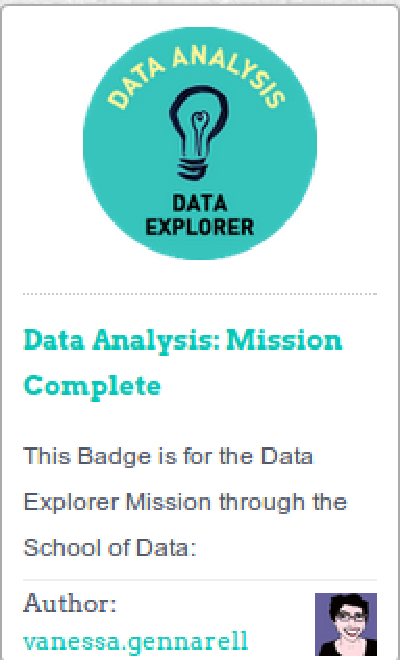
\includegraphics[width=0.40\linewidth]{badge}
\caption{Example of a badge offered at the P2P University}
\label{fig:badge}
\end{center}
\end{figure}

The P2P University offers all the necessary tools to create and award badges.
An example of a badge is shown in Figure~\ref{fig:badge}.

%The participants will watch a motivation video and a video tutorial.
%The tutorial will describe how to complete a simple project and will be complemented.
%Then, the participants have to collaborate to solve a challenge.
%The teachers offer a suggested challenge, but the participants are free to take other challenges that are relevant to them and to the course.
%Finally, the participants have to carefully document their works so that it can be evaluated, reproduced and discussed by the other participants.

%The first and the last unit are slightly different.
%In the first unit there is no project as the focus is on the presentation of the participants, the course itself and the discussion of the expectations on the course.
%The last unit is also special because the participants design, plan, execute and document their own project. 
%The courses finishes with an exhibition of the personal projects.

\subsection{In-person courses}
Besides the online offering, the course will also offered in-class for students registered at Universitat Pompeu Fabra.
Furthermore it will be possible to use the material for Summer Schools to promote the University and Bottom-up Initiatives.

\subsection{On-line platform}

As the goal is to reach everyone that has an interest on the construction of wireless sensor networks, the course will also be offered in the P2P University course platform.
This platform will be used to host the videos, written material and tools for discussion and feedback.

In hist keynote talk in Edulearn'13 in Barcelona, P2PU co-founder Philipp Schmidt explained that when they conceived P2PU they were looking for something different than Coursera or EdX.
The interest was in building something inexpensive, in a bottom-up fashion, using the resources already available on the web.

The peer-to-peer principles are summarized by the words ``Learning from the people, by the people. About almost anything''.

The P2P is built on strong principles. 
Their web highlights ``open'', ``community'' and ``peer learning''.
Technologies and processes are open to make it open to collaborate.
The organization is horizontal and driven by community discussions.
And everyone is invited to learn and teach using the platform.

The courses are not constricted to the tools of the platform itself. 
On the contrary, they make use of all the resources available in the web such as mailing lists, blogging, micro-blogging, instant messaging, forums and video-conferences, 

\subsection{Completion rate, statistics and scientific analysis of the experience}

One of the weaknesses of MOOCs are the low completion rates, typically below 10\%.
The reasons is that people registers for courses but do not have the necessary time and/or motivation to complete them.

The goal of the P2PU and the ``mechanicalmooc'' engine is to offer an engaging and enriching experience to the participants so that everyone benefits from the course.
Preetha Ram, which is involved in the ``mechanicalmooc'' has been quoted to say: ``We want to do more than sign up tens of thousands of students and have only a fraction succeed. Our goal is to have everyone who participates succeed''.

The system includes a logging and analytics system to keep tracks of clicks, emails and engagement in general.
All this data is available for researchers and a team lead by June Ahn (University of Maryland) is studying the data to find the best ways encourage the participation of all registered users \cite{ahn2013dop}

See \url{http://http://info.p2pu.org/research/} for further details.

\subsection{In-person Workshops and Meetings}

The participants in nearby locations will be encouraged to meet and gather to work together in the projects.
In-person collaboration provides a far richer experience than on-line work and helps to keep people participative and engaged.
Those that cannot meet in person will also be encouraged to get acquainted with their groups with presentation videos and/or other tools for team building.

\subsection{Additional Material}

\begin{itemize}
\item Robert Faludi ``Building Wireless Sensor Networks'' \cite{faludi2010bws}
\item Alejandro Andreu ``Open Sensor Network'' \cite{andreu2013osn}
\item Massimo Banzi ``Getting Started with Arduino'' \cite{banzi2009gsa}
\end{itemize}


%------------------------------------------------

\section{Work Plan}

\begin{enumerate}
    \item Identifying and specifying the course goals, the assignments and projects to learn and achieve such goals as well as the evaluation criteria. October 2013.
	\item Scripting of the course: preparation of the course structure including units segmentation, number/length of videos per unit, assignments and quiz dynamics and evaluation, feedback and collaboration management; and final project evaluation. November 2013.
	\item Preparation of the written guide: there is already a guide for the in-class course, therefore this new adapted guide should take advantage of on-line resources (video, comments, etc.). December 2013.
    \item Preparation of the quizzes. 
    Embedded googleforms will be used for the quizzes. January 2014.
    \item Preparation of the badges using the P2P University tools. February 2014.
	\item Setting up the P2P University on-line platform: based on the course script, this task will configure the platform accordingly. February 2014.
	\item Shooting and producing the videos: this final task aims at shooting the videos according to what was designed in the course script and configured in the P2P University platform. March 2014.
\end{enumerate}


\begin{figure}
\begin{center}
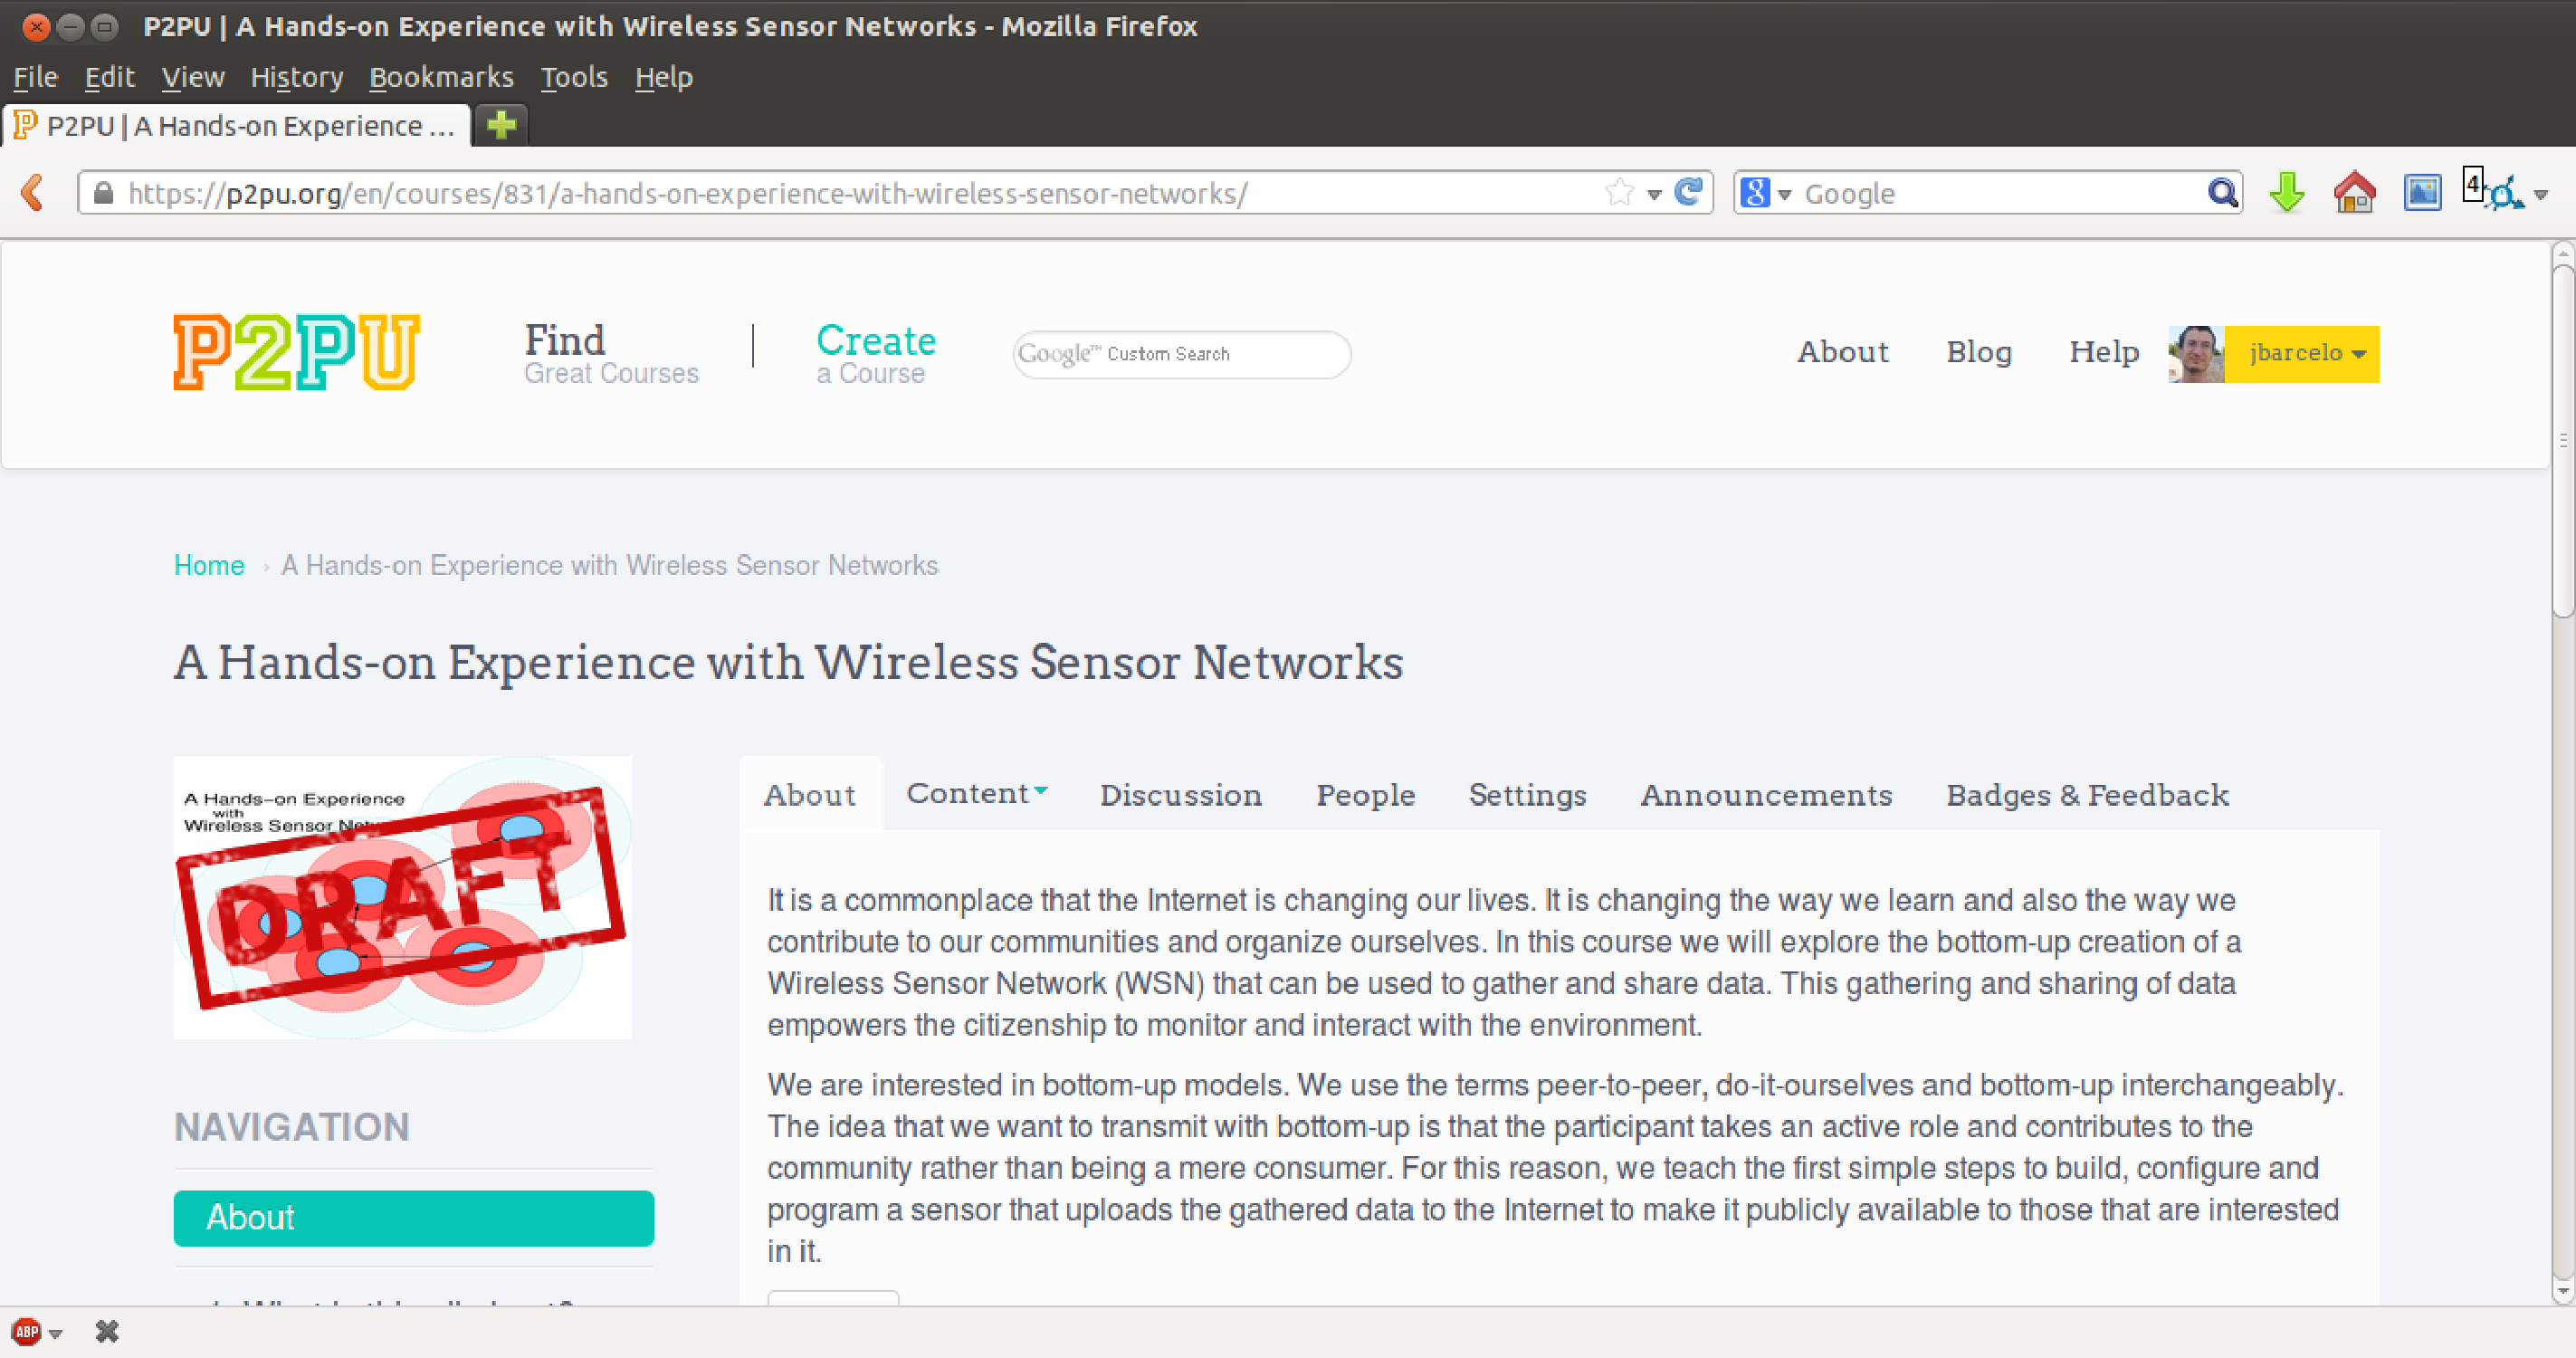
\includegraphics[width=1.00\linewidth]{screenshot}
\caption{A screenshot of a draft of the course at P2P University}
\label{fig:SCK}
\end{center}
\end{figure}

% \begin{itemize}
% \item Scripting of the course: Preparation of detailed scripts of the content of the videos, the guide and the requirements for the online platform.
% \item Shooting and producing the videos: The videos will be shot and produced according to the script.
% \item Preparation of the written guide: There is already a guide for the in-class course, but it needs to be adapted to the on-line course.
% \item Setting up the P2P University on-line platform: This task involves the actual creation and configuration of the online course.
% \end{itemize}

%\begin{figure}
%\begin{center}
%\includegraphics[width=0.40\linewidth]{video}
%\caption{It is necessary to shoot videos with step-by-step instructions to build the projects or complete the assignments.}
%\label{fig:video}
%\end{center}
%\end{figure}
%\begin{figure}
%\begin{center}
%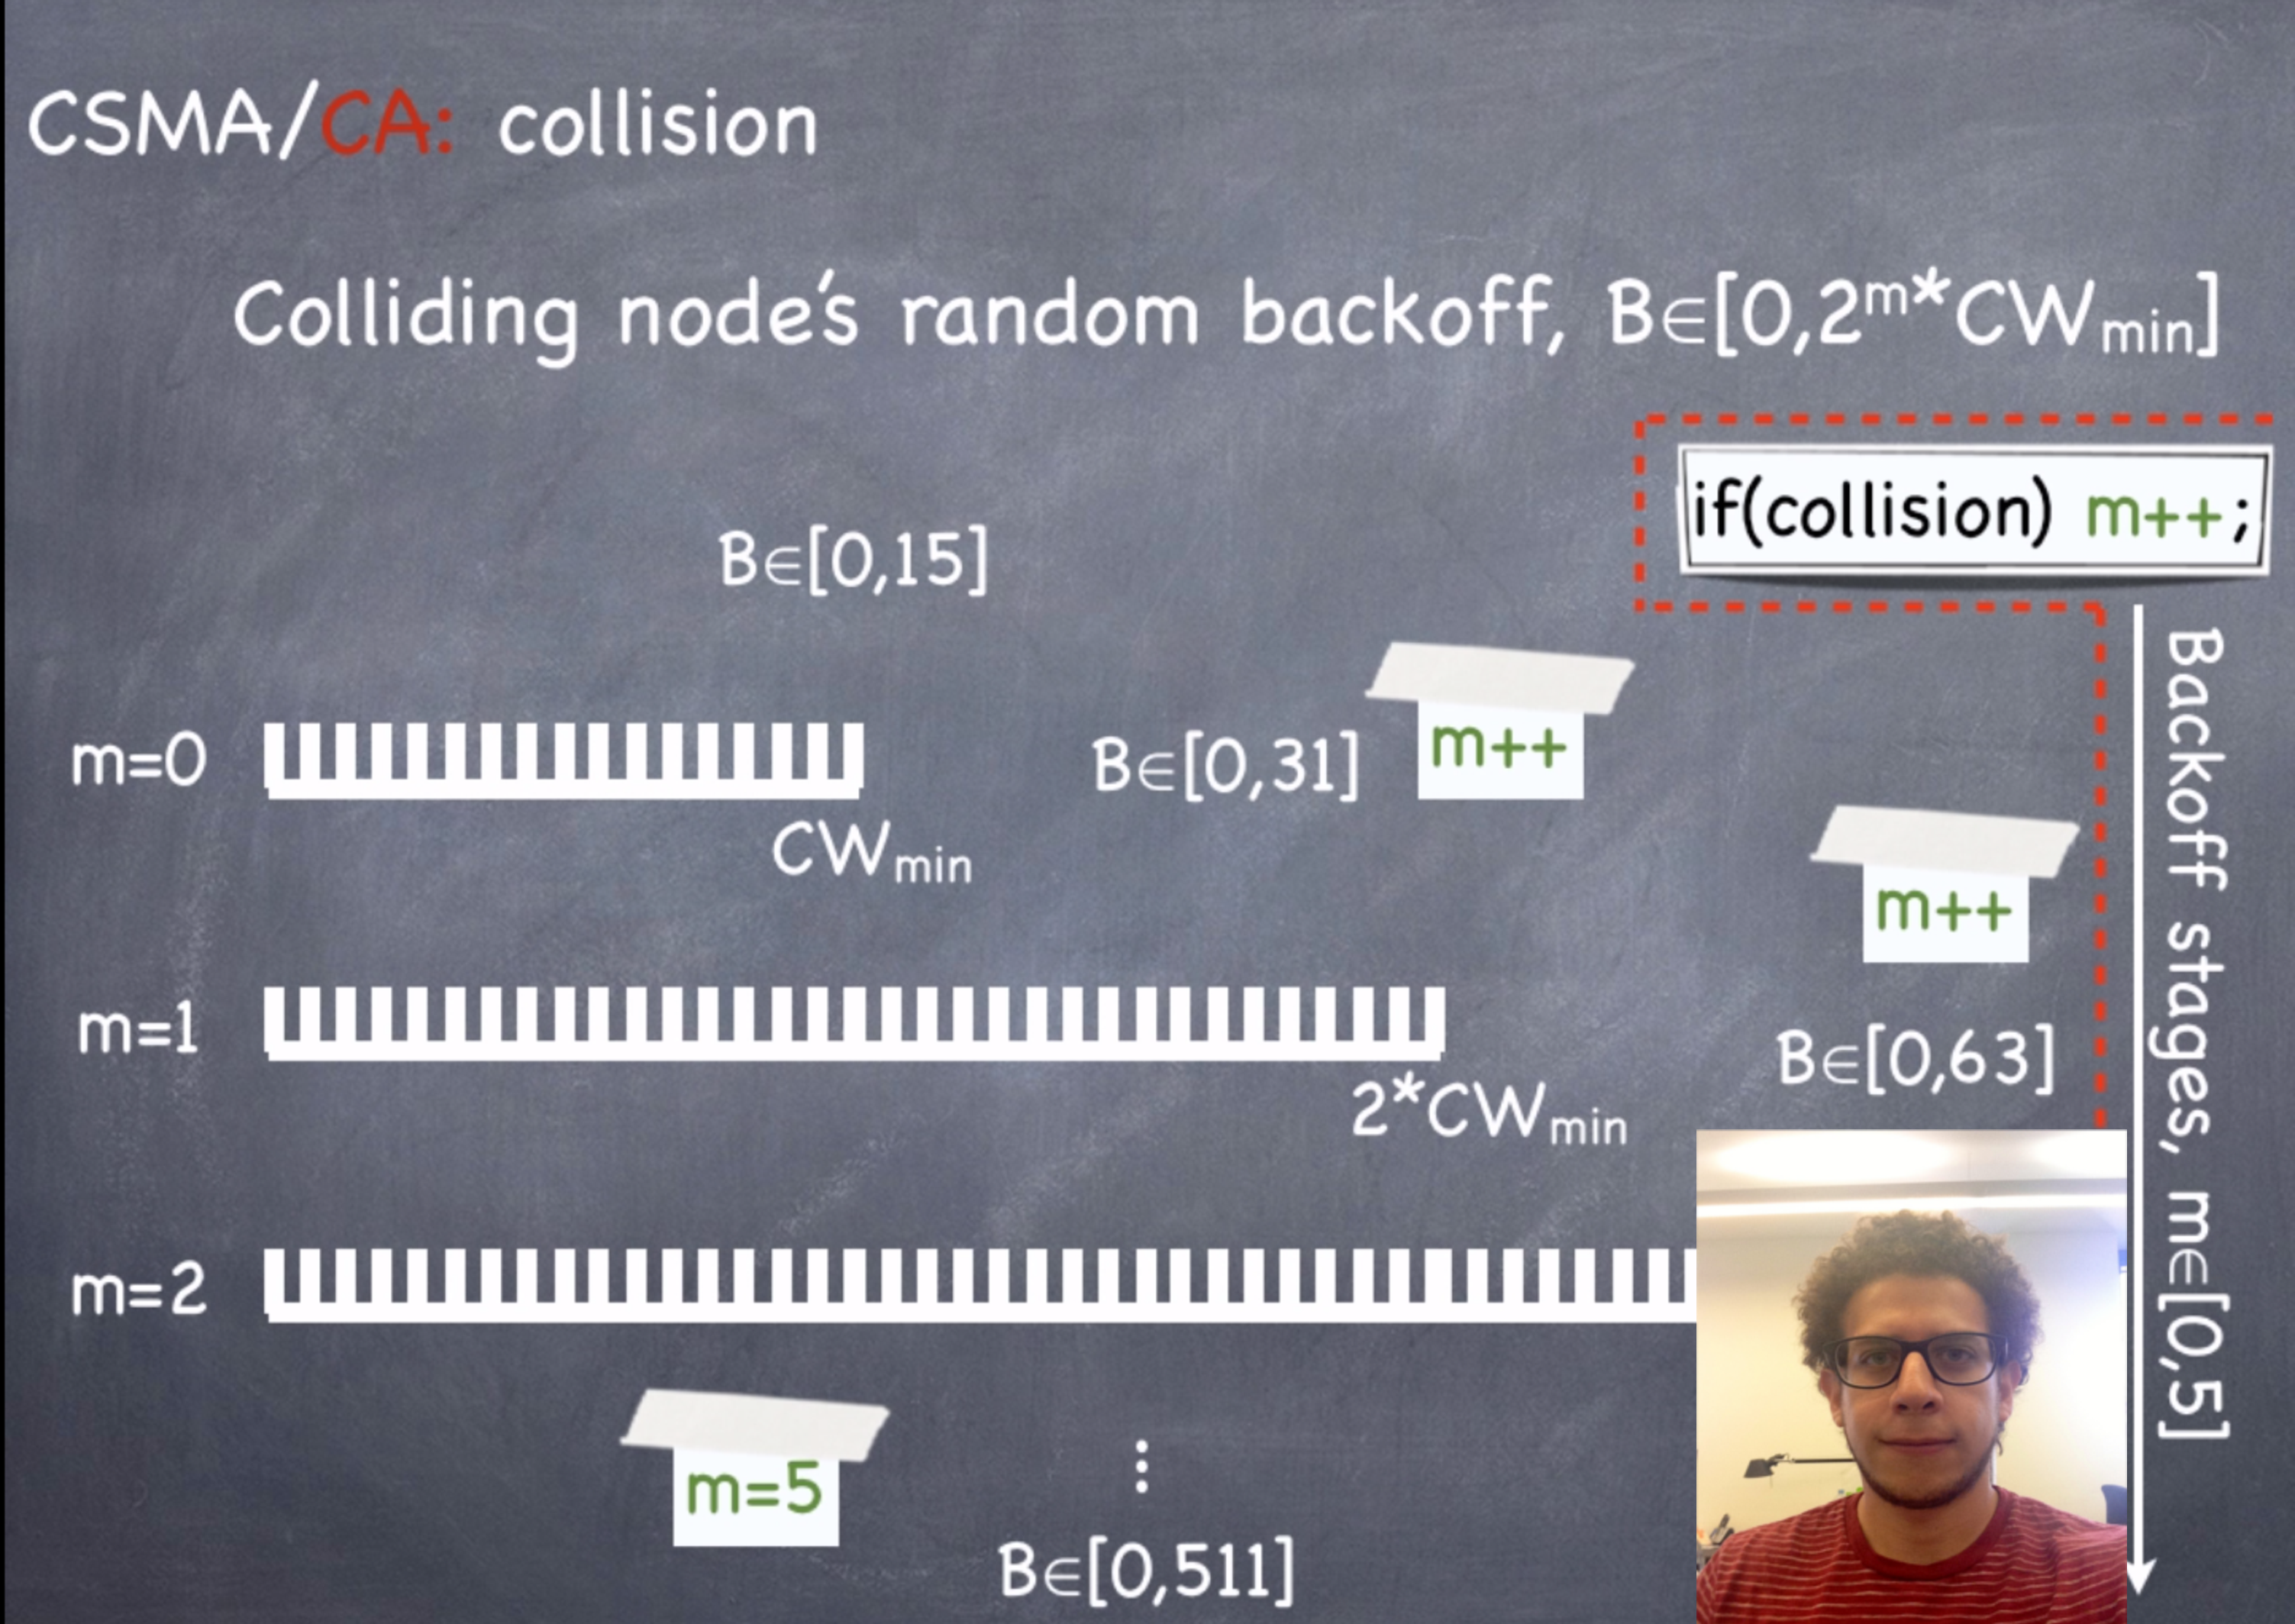
\includegraphics[width=0.40\linewidth]{lesson}
%\caption{Some video lessons will show the teacher's face over supporting slides.}
%\label{fig:lesson}
%\end{center}
%\end{figure}

\subsection{Coordination tools}
The tools will be the typical for collaborative projects:
A mailing list for day-to-day progress and weekly meetings.
Also IRC discussions as needed.
Agile methodologies, \emph{Trello} and \emph{Wiggio} will also be considered for project and group management.

%------------------------------------------------

\section{Results and Impact}

This course builds upon successful experiences. There is already an existing in-person course that received very good feedback from the students.
The laboratory guide of the course is available in \texttt{github} (\url{https://github.com/jbarcelo/WSNs_lecture_notes}) making it easy for everyone to contribute.
We also published the guide in \texttt{scribd} in late July (\url{http://www.scribd.com/doc/156136472/A-course-on-Wireless-Sensor-Networks-WSNs}) and was read more than 200 times in August.

Also, the idea of bottom-up smart cities implemented by Smart Citizen was applauded in Kickstarter and received over \$60,000 in crowdfunding. 

The hardware used in the course includes the Digi XBee and the Arduino board. 
This tandem was also used in the best-selling book by Rober Faludi ``Building Wireless Sensor Networks''.
Arduino is a first choice platform for those interested in an introduction to electronics and micro-controllers.
More than one million Arduino have been sold, confirming the success of their open business model.

The main goal of this course is to strengthen the community by teaching very basic skills to a large audience. After completing the course, the participants will be able to continue on their own with more advanced projects. 

It is a basic digital education for everyone. People with no or little background in technology will make their first steps into programming, electronics, and sensing projects.

Students successfully completing this course will posses the basic tools to contribute to the creation of bottom-up smart cities.

\subsection{Results obtained so far}

By simply creating this document and discussing it with the involved communities on the Internet, we have received many inputs, ideas, and encouragement that has helped to further shape the idea.

\subsection{Eternal work-in-progress}

Many collaborative projects never come to an end.
These projects keep evolving and improving, and the actual direction of the evolution is highly dependant of the people that is working in it in every moment.
The idea is to keep gathering feedback from the participants and use that information to continuously improve the course.
For this reason it is very important that everyone involved does not feel like a simple ``consumer''.
The goal is that the participants are also the ``makers'' of the course and everyone learns from everyone in peer-to-peer way.

% This course builds upon successful experiences. There is already an existing course that received very good feedback from the students. There is also a degree thesis by one of the students that was presented in Battlemesh, Aalborg University, and attracted the attention of the P2P Foundation.
% 
% The idea of bottom-up smart cities implemented by Smart Citizen was applauded in kick starter and received over \$60,000 in crowdfunding. The hardware used in the course is the XBee that was also used in the best-selling book by Rober Faludi “Building Wireless Sensor Networks”. More than one million Arduino have been sold confirming the success of their open business model.
% 
% The main goal of this course is to strengthen the community by teaching very basic skills to a large audience. After completing the course, the participants will be able to continue on their own with more advanced projects. It is a basic digital education for everyone. People with no or little background in technology will be do the first steps in programming, electronics, and sensing projects.
% 
% People that have taken the course will be able to contribute to the creation of bottom-up smart cities.



%------------------------------------------------

\section{Teaching Plan}

\subsection{Concepts and competences acquired in the course}
\begin{itemize}
\item Bottom-up, peer-to-peer and community-oriented collaboration models
\item Sensors, actuators, sensor networks, open data, smart cities
\item Very basic electronics
\item Very basic microprocessor programming
\item Configuration of Digi XBee
\item ZigBee communication
\end{itemize}


\subsection{Weekly organization}
\begin{enumerate}
\item Presentation of the participants, presentation of the course, motivation to take the course, dream about a personal project.
\item Introduction to Arduino. Arduino IDE. Input/output. \\\underline{Lab assignment}: Blinking LED project.
\item Introduction to XBee. Basic configuration of AT mode. \\\underline{Lab assignment}: ZigBee chat project.
\item Basic interaction. Make a measurement and react. \\\underline{Lab assignment}: Wireless Sunset Sensor project.
\item Open data. The importance of sharing the data. Open data platforms. \\\underline{Lab assignment}: Taking measures with a sensor and uploading them to the Internet.
\end{enumerate}

Motivating videos:
\begin{itemize}
\item Do-it-ourselves, Bottom-up, Sensors, Smart Cities, Smart Cities Kit:
Laia Albo (UPF), Someone from P2PF (Michel Bauwens?), Tiberius Brastaviceanu (Sensorica), Guillem Camprodon and Tomas Diez (FABLAB), Alex Posada (MID)

\item Arduino (Blinking LED):
Someone from Arduino - David Mellis?, (Jaume)

\item XBee (Chat):
Someone from Digi - Robert Faludi?, (Luis)

\item Interaction design (Sunset Sensor):
Alex Posada (Luis)

\item Open Data, Open Data platforms (Internet thermometer):
Albert Domingo, Manuel Palacin, (Alejandro Andreu)
\end{itemize}


%------------------------------------------------

\chapter{Team}

\section{Lead teacher}
\begin{itemize}
\item Jaume Barcelo (Universitat Pompeu Fabra): He is a lecturer at Universitat Pompeu Fabra where he takes part in the Wireless Sensor Network course. He has also taught at Universidad Carlos III de Madrid were he collaborated with the opencourseware experience that published the class materials online. Together with Luis Sanabria, he has prepared the basic laboratory guide for the Wireless Sensor Networks course that has been shared with the Internet community. Jaume has taught more than 20 courses at the graduate and undergraduate level at two universities. Visit www.jaumebarcelo.info for more information.
\begin{figure}
\begin{center}
\includegraphics[width=0.200\linewidth]{jaume}
\caption{Jaume Barcelo}
\label{fig:jaume}
\end{center}
\end{figure}
\end{itemize}


\section{Other members of the team}
\begin{itemize}
\item Laia Albo (Universitat Pompeu Fabra): She is a research technician at Telefonica-UPF chair ``Social Innovation in Education''. Audiovisual Systems Engineer from the University Pompeu Fabra, she has worked in the Teaching Quality and Innovation Support Unit (USQUID) of the Polytechnic School of the UPF to support the project linked to the creation of educational videos for academic support (both for teachers and students).
\begin{figure}
\begin{center}
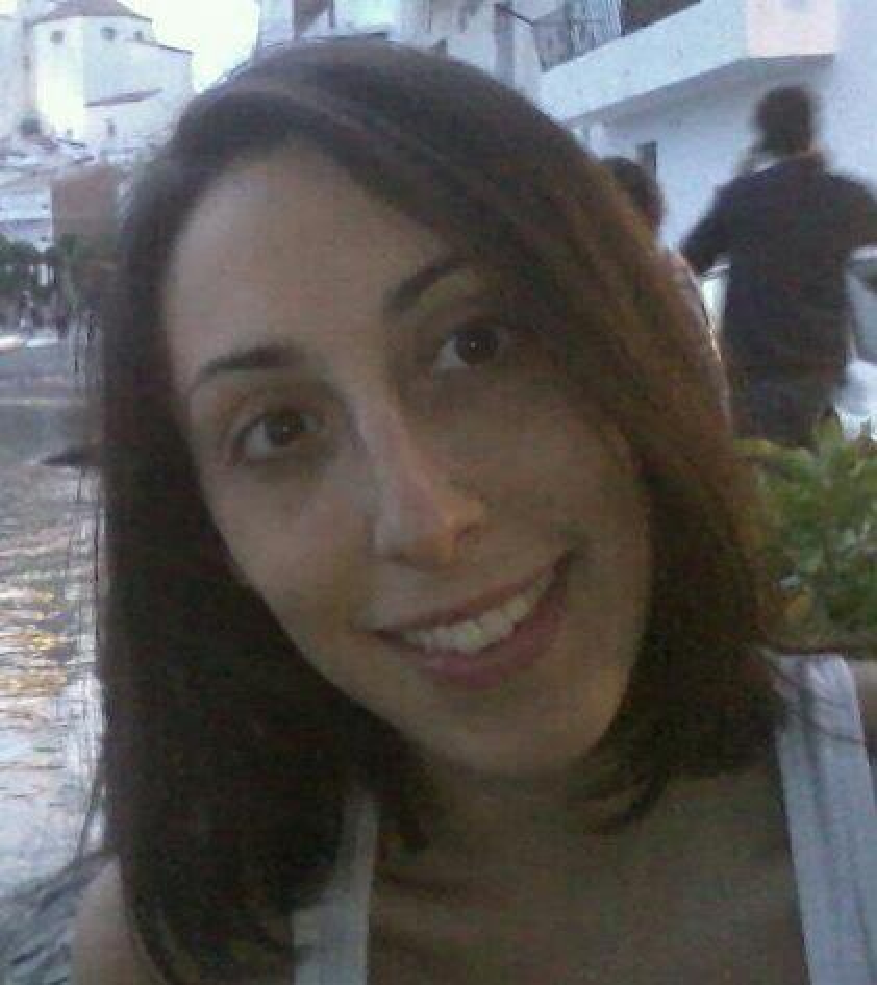
\includegraphics[width=0.200\linewidth]{laia}
\caption{Laia Albo}
\label{fig:jaume}
\end{center}
\end{figure}
\item Alejandro Andreu (Universitat Pompeu Fabra): He completed his degree on Computer Communications with a thesis entitled ``Open Sensor Networks''. He has also contributed to the Smart Citizen Kit project.
\begin{figure}
\begin{center}
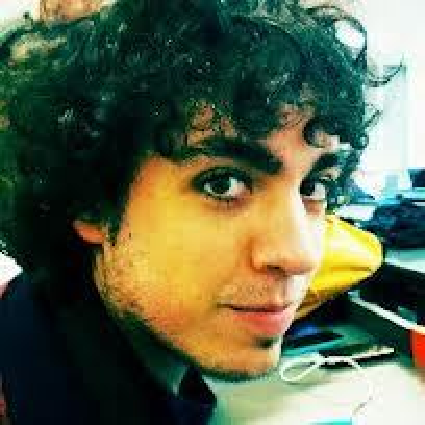
\includegraphics[width=0.200\linewidth]{alejandro}
\caption{Alejandro Andreu}
\label{fig:jaume}
\end{center}
\end{figure}
\item Someone from Arduino - David Mellis? (Arduino)
\item Someone from P2PF - Michel Bauwens? (P2P Foudation)
\item Tiberius Brastaviceanu (Sensorica): He is founder, active member, coordinator, facilitator, engineer and product designer at Sensorica.
\begin{figure}
\begin{center}
\includegraphics[width=0.200\linewidth]{Tiberius}
\caption{Tiberius Brastaviceanu}
\end{center}
\end{figure}
\item Guillem Camprodon (FabLab Barcelona): He is a researcher at the Institut d'Arquitectura Avancada de Catalunya (IAAC). He participates in the Smart Citizen Kit project as the main responsible for integration and project development (hardware and software).
\item Tomas Diez (FabLab Barcelona): He is the director of FabLab Barcelona at the Institut d'Arquitectura Avancada de Catalunya (IAAC) and co-founder of the Smart Citizen Kit initiative. Tomas is also part of the master programs taught at IAAC.
\begin{figure}
\begin{center}
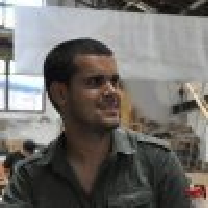
\includegraphics[width=0.200\linewidth]{tomas}
\caption{Tomas Diez}
\end{center}
\end{figure}
\item Albert Domingo (Universitat Pompeu Fabra):
He is currently a Ph.D. candidate at the Networking and Strategies (NeTS) group at UPF. He has also been a visitor with the Advanced Network Architecture group at MIT.

He is a teaching assistant in a course about networking protocols. His research interests include Super-Wifi communications, Open Data, Big Data, public administration data and regulation. He participates in the 'Commons for Europe' and 'Open Cities' European projects. 
\begin{figure}
\begin{center}
\includegraphics[width=0.200\linewidth]{Albert}
\caption{Albert Domingo}
\end{center}
\end{figure}
\item Someone from Digi - Robert Faludi? (Digi International)
\item Vanessa Gennarelli (P2P University): She is Learning Lead at P2PU.
\begin{figure}
\begin{center}
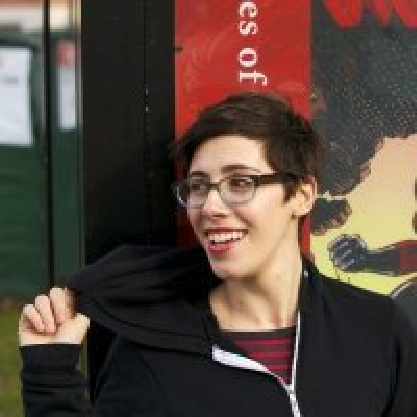
\includegraphics[width=0.200\linewidth]{vanessa}
\caption{Vanessa Gennarelli}
\end{center}
\end{figure}
\item Luis Sanabria-Russo (Universitat Pompeu Fabra)
\begin{figure}
\begin{center}
\includegraphics[width=0.200\linewidth]{luis}
\caption{Luis Sanabria-Russo}
\label{fig:luis}
\end{center}
\end{figure}
\item Manuel Palacin (Universitat Pompeu Fabra)
\item Alex Posada (Media Interaction Design Lab): He is the founder and CEO at Media Interactive Design (MID) and also coordinates the Interaction Lab at hangar.org . Alex teaches in the Master of Advanced Architecture and the Master of Advanced Interaction at the Institut d'Arquitectura Avancada de Catalunya (IAAC). Alex is a co-founder of the Smart Citizen Kit initiative.
\begin{figure}
\begin{center}
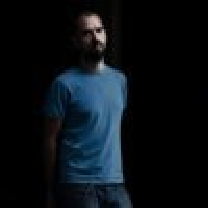
\includegraphics[width=0.200\linewidth]{alex}
\caption{Alex Posada}
\end{center}
\end{figure}
\item And you, if you want. Everyone is invited to join the team and collaborate.
\end{itemize}

\bibliographystyle{apalike}
\bibliography{my_bib}

\end{document}
